\documentclass[a4paper,UKenglish,cleveref,autoref,thm-restate,anonymous]{lipics-v2021}

\usepackage{amsmath}
\usepackage{amssymb}
\usepackage{booktabs}
\usepackage{tikz}
\usetikzlibrary{arrows.meta,decorations.pathreplacing}
\usepackage{array}

\bibliographystyle{plainurl}

\title{How Much Algebra Does a Beatpath Need? Schulze's Guarantees and the Bottleneck Semirings}

\titlerunning{How Much Algebra Does a Beatpath Need?}

\author{Mina Cyrus}{Department of Computer Science, Swansea University,
  Swansea, UK}{m.a.cyrus@swansea.ac.uk}{}{}
%\author{Dirk Pattinson}{Department of Computer Science, Australian National
%  University, Canberra, Australia}{dirk.pattinson@anu.edu.au}{}{}
%\author{Nobuko Yoshida}{Department of Computer Science, University of
%  Oxford, Oxford, UK}{nobuko.yoshida@cs.ox.ac.uk}{}{}
%\author{Mukesh Tiwari}{Department of Computer Science, Swansea University,
%  Swansea, UK}{mukesh.tiwari@swansea.ac.uk}{}{}

\authorrunning{M. Cyrus, D. Pattinson, N. Yoshida, and M. Tiwari}

\Copyright{Mina Cyrus, Dirk Pattinson, Nobuko Yoshida, and Mukesh Tiwari}

\ccsdesc[500]{Theory of computation~Algebraic semantics}
\ccsdesc[300]{Theory of computation~Logic and verification}
\ccsdesc[300]{Mathematics of computing~Graph algorithms}

\keywords{Semirings, Kleene star, algebraic path problem, bottleneck semiring,
social choice, interactive theorem proving}

\category{Track B: Automata, Logic, Semantics, and Theory of Programming}

\newcommand{\Mstar}{M^{\ast}}
\newcommand{\clo}[2]{#1^{\ast\langle #2\rangle}}
\newcommand{\rocq}{\textsc{Rocq}}
\newcommand{\Trop}{\mathbb{T}}
\newcommand{\Diam}{\mathbb{D}}
\newcommand{\Bool}{\mathbb{B}}
\newcommand{\anonrepo}{https://anonymous.4open.science/r/Semiring_graph_algorithm-000E}
\newcommand{\rocqfile}[2]{\href{\anonrepo/#1}{\textcolor{blue}{\texttt{#2}}}}
\newcommand{\proofat}[2]{{\footnotesize\itshape\rocq{} proof: \rocqfile{#1}{#2}}}
\newcommand{\rocqrelated}[1]{{\footnotesize\itshape Related \rocq{} files: #1}}
\newcommand{\rowlab}[1]{\textbf{#1}}

\begin{document}

\maketitle

\begin{abstract}
The Schulze method is a widely used single-winner election method based on
\emph{beatpaths}. One alternative beats another when the strongest path
from the first to the second is stronger than the strongest path back,
where the strength of a path is the strength of its weakest link. The
matrix of strongest paths is the Kleene star of the pairwise matrix over
the semiring $\langle \mathbb{N}^{\infty}, \max, \min\rangle$, so every
one of Schulze's guarantees is a theorem about that semiring.

We interpret those guarantees over an arbitrary semiring and ask, for each
one, which algebraic axioms its proof uses. They sort into four levels.
Neutrality holds over any semiring. The Pareto condition and monotonicity
need only \emph{boundedness}, that $1 + a = 1$. The Smith criterion and
Condorcet consistency need in addition \emph{selectivity}, that $x + y$ is
always $x$ or $y$, and each fails without it. The criteria that compose two
beatpaths need in addition the \emph{meet property}, that $a \cdot b$ is
the greatest lower bound of $a$ and $b$. Reversal symmetry, in its
relation-level form, sits outside the hierarchy: it needs only
commutativity.

At the top level the converse holds as well. Over a bounded semiring with
decidable equality, the beatpath relation is transitive for every profile
exactly when the semiring is selective and has the meet property, and a
semiring with both is $\max$ and $\min$ on a total order. Schulze's two
operations are therefore the only ones that guarantee an ordering; the only
freedom left is the totally ordered scale on which strengths are measured.
The same two axioms characterise winner existence and independence of
clones, so those two guarantees are the same condition on the semiring.
Every result is machine-checked in \rocq{}.
\end{abstract}

\section{Introduction}\label{sec:intro}
The Schulze method~\cite{schulze2011new} ranks alternatives by
\emph{beatpaths}. From a profile of ballots, one derives a matrix $M$ of
pairwise link strengths. A path $a = c_0, c_1, \dots, c_k = b$ has the
strength of its weakest link, and alternative $a$ outranks $b$ when the
strongest path from $a$ to $b$ beats the strongest path from $b$ to $a$.
Here strongest means $\max$ and weakest means $\min$. The matrix of
strongest paths is then exactly the Kleene star
\[
  \Mstar \;=\; I \oplus M \oplus M^{2} \oplus \cdots
\]
of $M$ over the semiring $\langle \mathbb{N}^{\infty}, \max, \min\rangle$,
and the method's output follows from the comparison
\[
  a \succ b \quad\text{iff}\quad \Mstar_{ba} < \Mstar_{ab}
\]
taken in that semiring's natural order.

Now change the arithmetic from $\langle \mathbb{N}^{\infty}, \max,
\min\rangle$ to $\langle \mathbb{N}^{\infty}, \min, +\rangle$ and keep
everything else. A path now has the \emph{sum} of its links as its
strength, read as a cost, and the best path is the cheapest one. Then
$\Mstar$ holds shortest distances, and $a \succ b$ says that $a$ reaches
$b$ more cheaply than $b$ reaches $a$. Only the two operations have
changed, and three alternatives are already enough to make the method
fail.

\begin{example}[One profile, two semirings]\label{ex:tropical}
Take three alternatives and three voters ranking them cyclically: one votes
$a > b > c$, one votes $b > c > a$, and one votes $c > a > b$. Pairwise, $a$
beats $b$ two votes to one, $b$ beats $c$ two to one, and $c$ beats $a$ two
to one, so the majority relation is a cycle and there is no Condorcet
winner.

Over $\langle \mathbb{N}^{\infty}, \max, \min\rangle$, let $M_{ij}$ be the
number of voters ranking $i$ above $j$, with rows and columns indexed
$a,b,c$ and $0$ on the diagonal:
\[
  M \;=\;
  \begin{pmatrix}
    0 & 2 & 1 \\
    1 & 0 & 2 \\
    2 & 1 & 0
  \end{pmatrix},
  \qquad
  \Mstar \;=\;
  \begin{pmatrix}
    \infty & 2 & 2 \\
    2 & \infty & 2 \\
    2 & 2 & \infty
  \end{pmatrix}.
\]
The direct link from $b$ to $a$ has strength $1$, but the detour
$b \to c \to a$ has strength $\min(2,2) = 2$, which matches the direct link
from $a$ to $b$; the other two pairs behave the same way. Every
off-diagonal entry of $\Mstar$ is therefore $2$, no comparison
$\Mstar_{ba} < \Mstar_{ab}$ is strict, and $\succ$ is empty. No alternative
beats another, so all three are winners.

Now keep the profile and change the semiring to $\langle \mathbb{N}^{\infty},
\min, +\rangle$, charging each link the number of voters opposed to it, so
that each hop forward round the cycle $a \to b \to c \to a$ costs $1$ and
each hop back costs $2$. The detour from $b$ to $a$ now costs $1 + 1 = 2$,
no better than the direct hop back, so the cheapest route from $b$ to $a$
costs $2$ while the direct hop from $a$ to $b$ costs $1$, and $a \succ b$.
By symmetry $b \succ c$ and $c \succ a$. The cycle survives the closure as
a cycle of \emph{strict} wins, every alternative is beaten by another, and
the winner set is empty.
\end{example}

The two halves of \Cref{ex:tropical} run the same ballots through the same
construction and disagree completely. The guarantee that Schulze's method
returns an ordering with a winner therefore does not come from the beatpath
idea alone; it comes from $\max$ and $\min$. That is one guarantee, and
Schulze's method has many others. Raising a candidate's support never harms
it (monotonicity). A candidate who beats every other head to head is always
elected (Condorcet consistency). Every winner comes from the smallest set
of candidates that beats everyone outside it (the Smith criterion). And
there are several more.

It has long been known that the closure construction itself is generic:
transitive closure, shortest paths, and widest paths are all instances of
one algorithm run over different
semirings~\cite{carre1971algebra,lehmann1977,10.5555/1386688,baras2022path}.
To our knowledge, though, social choice theory has never been carried to
that same level of generality. This paper does so. For each of Schulze's
guarantees we ask the same question: which algebraic axioms does its proof
actually need?

\subparagraph*{Our contributions.}
Interpreting the social choice theory over a semiring turns each of
Schulze's criteria into a statement about that semiring. Each such
statement then holds or fails depending on the axioms the semiring
satisfies, so the criteria stop being a flat list and acquire a structure.
Describing that structure takes four definitions: \emph{idempotence},
\emph{boundedness}, \emph{selectivity}, and the \emph{meet property}. Our
contributions are the following.

\begin{enumerate}
\item \textbf{A classification of Schulze's criteria by algebraic strength}
(\Cref{sec:classification}). We prove each criterion at the weakest level
of structure at which we can establish it. The levels form a hierarchy in
which each adds one axiom to the one below: neutrality needs no assumption
at all (Level 0); weak Pareto and monotonicity need boundedness (Level 1);
the Smith criterion, Smith-IIA, Condorcet consistency, and the resolution
step need selectivity in addition (Level 2); and transitivity of $\succ$,
winner existence, independence of clones, reversal symmetry, prudence, and
the MinMax set need the meet property in addition (Level 3).
\Cref{tab:classification} summarises the classification.

\item \textbf{An exact characterisation at Level 3}
(\Cref{sec:characterisation}). The two axioms of Level 3 are not merely
enough; they are exactly what transitivity costs. Over a bounded semiring
with decidable equality and at least three alternatives, $\succ$ is
transitive for every matrix if and only if the semiring is selective and
has the meet property, and a semiring with both is $\max$ and $\min$ on a
total order (\Cref{thm:structure}). Schulze's two operations are therefore
not one workable choice among several: they are the only one, and the only
freedom left is which totally ordered scale the strengths are drawn from.
The same two axioms characterise winner existence
(\Cref{thm:winnerchar}) and independence of clones (\Cref{thm:clonechar}),
so on any semiring those two guarantees stand or fall together.

\item \textbf{Sharpness} (\Cref{sec:sharp}). Each axiom is necessary on
its own, not merely jointly. The tropical semiring is selective but lacks
the meet property, and already at three alternatives it admits a matrix
with no winner. The four-element diamond lattice has the meet property but
is not selective, and it admits one at four alternatives but, as a machine
check of all $4^{9}$ cases shows, at no fewer. The diamond also refutes
every Level 2 criterion, so that level is sharp too.

\item \textbf{A complete mechanisation} in \rocq{}
(\Cref{sec:formalisation}). A classification by \emph{weakest} hypothesis
is a claim about what a proof does \emph{not} use, and informal argument
gets exactly this kind of claim wrong, because an unused hypothesis costs
the author nothing and is invisible to the reader. Every entry in our table
is therefore backed by a \rocq{} proof that typechecks without the
hypotheses we omit. The full development, more than $20{,}000$ lines of
\rocq{}, is available in an
\href{https://anonymous.4open.science/r/Semiring_graph_algorithm-000E/README.md}{\textcolor{blue}{anonymous proof repository}} with
\href{https://anonymous.4open.science/r/Semiring_graph_algorithm-000E/docs/toc.html}{\textcolor{blue}{documentation}}.
\end{enumerate}

\subparagraph*{How the paper is arranged.}
\Cref{sec:prelim} fixes the algebra and \Cref{sec:framework} the beatpath
construction over it, including the one point at which the closure has to
be reconciled with what the method actually prescribes.
\Cref{sec:classification} states the classification.
\Cref{sec:characterisation} proves that the top of the hierarchy is exact
and that neither of its two axioms can be traded for the other.
\Cref{sec:formalisation} describes the \rocq{} development,
\Cref{sec:related} places the work beside the algebraic path and verified
social choice literature, and \Cref{sec:conclusion} concludes.

\section{Background}\label{sec:prelim}

Two ingredients are needed before any criterion can be stated. The first
is the semiring: it supplies the two operations that combine link
strengths, and its \emph{natural order} is what turns those strengths into
comparisons, so that saying one beatpath is stronger than another means
something. The second is the closure: matrices over a semiring form a
semiring in their own right, and the Kleene star of a matrix collects the
strengths of all paths at once. Neither is new, and the reader who knows
the algebraic path problem will recognise both; we set them out because
the whole paper turns on which of their axioms each later proof uses.

\subsection{Semirings and the Natural Order}

\begin{definition}[Semiring]
A \emph{semiring} is a tuple $R = \langle R, +, \cdot\,, 0, 1\rangle$ where
$\langle R,+,0\rangle$ is a commutative monoid, $\langle R,\cdot\,,1\rangle$ is
a monoid, multiplication distributes over addition on both sides, and
$0\cdot a = a \cdot 0 = 0$. It is \emph{idempotent} if $a+a=a$,
\emph{commutative} if $\cdot$ is, and \emph{bounded} if $1 + a = 1$ for all
$a$.
\end{definition}

Boundedness says $1$ absorbs $+$; it implies idempotence and is the standing
assumption throughout. In the intended reading it is not a restriction but a
fact: the empty path should be unbeatable.

\begin{definition}[Natural order]
For an idempotent semiring put $a \leq b \iff a+b=b$, and write $a<b$ for
$a\leq b$ with $a \neq b$.
\end{definition}

\begin{lemma}\label{lem:natural}
On an idempotent semiring the natural order is a partial order, $+$ is its
join, and multiplication is monotone in both arguments. If $R$ is bounded then
$0$ is least, $1$ is greatest, and $a\cdot b \leq a$ and $a\cdot b \leq b$.
\proofat{algorithm/OrelN.v}{OrelN.v}
\end{lemma}

\begin{proof}
Reflexivity is the idempotence axiom itself, since $a \leq a$ unfolds to
$a + a = a$. The proofs of transitivity, antisymmetry, and monotonicity are
each a one-line rewrite; for transitivity, $a+b=b$ and $b+c=c$ give
$a + c = a + (b + c) = (a+b) + c = b + c = c$, and the other two are
similar. For the bounded clauses, $0+a=a$ and $1+a=1$ give the extremes,
and $a\cdot b + a = a(b+1) = a$ gives $a\cdot b \leq a$, symmetrically on
the other side.
\end{proof}

The last clause separates this setting from arbitrary semirings: here
multiplication only loses strength. That is the right reading when a
product is the strength of a composite path, and it fails in
$\langle \mathbb{N}, +, \times\rangle$, which is therefore out of scope.

\begin{definition}[Selectivity, meet property]\label{def:sel-meet}
$R$ is \emph{selective} if $x+y \in \{x,y\}$ for all $x,y$. It has the
\emph{meet property} if $m \leq a$ and $m \leq b$ imply $m \leq a\cdot b$.
\end{definition}

Selectivity is exactly totality of the natural order, and with
\Cref{lem:natural} the meet property says $a\cdot b$ is the greatest lower
bound of $\{a,b\}$.

\subsection{Matrices and the Kleene Star}

\begin{definition}[Matrices and the star]
Fix a finite set $A$ of alternatives, $|A| = n$. A \emph{matrix} over $R$
assigns to every ordered pair of alternatives a strength, $M : A \times A
\to R$, written $M_{ij}$. Matrices form a semiring under entrywise
addition $(M\oplus N)_{ij} = M_{ij}+N_{ij}$ and the usual product
$(M\otimes N)_{ij} = \sum_k M_{ik}\cdot N_{kj}$; the identity $I$ carries
$1$ on the diagonal and $0$ elsewhere. The \emph{star} of $M$ is the
series
\[
  \Mstar
  \;=\; \bigoplus_{ 0 \leq k} M^{k}
  \;=\; I \oplus M \oplus M^{2} \oplus \cdots .
\]
\end{definition}

Entrywise, $(M^{k})_{ij}$ joins the strengths of all walks of length
exactly $k$ from $i$ to $j$, so $\Mstar_{ij}$ joins the strengths of all
walks from $i$ to $j$, of every length. (A \emph{walk} may revisit an
alternative; a \emph{path} may not. \Cref{sec:walks} shows the distinction
does not matter here.) In a general semiring this join is an infinite sum
and need not exist; over $\langle \mathbb{N}, +, \times\rangle$ the powers
simply grow.

Boundedness is what brings the series to a fixed point. Over a bounded
semiring, a walk of length $n$ or more revisits some alternative, and
cutting out the cycle between the two visits leaves a shorter walk of at
least the same strength, because products only lose strength
(\Cref{lem:natural}). Every power beyond $M^{n-1}$ is therefore dominated
by the earlier ones and adds nothing to the join, so the series stabilises
at stage $n-1$:
\[
  \Mstar \;=\; I \oplus M \oplus M^{2} \oplus \cdots \oplus M^{n-1}
  \;=\; (M \oplus I)^{n-1}.
\]
The second equality uses idempotence: expanding $(M \oplus I)^{n-1}$ by
distributivity produces each $M^{k}$ many times over, and $a + a = a$
merges the duplicates.

The development takes this truncated sum as the definition of the closure.
That is the standard definition in the algebraic path literature, where
the closure over a suitably stable semiring is obtained at a finite
power~\cite{carre1971algebra,lehmann1977}, and the name Kleene star is
earned: the truncation satisfies $\Mstar = I \oplus (M \otimes \Mstar)$,
the defining equation of the star for matrices. The truncation remains
meaningful even without boundedness, and the one bare-semiring result,
neutrality, is a statement about it.
\rocqrelated{\rocqfile{algorithm/MatN.v}{MatN.v},
\rocqfile{algorithm/SemimoduleN.v}{SemimoduleN.v}, and
\rocqfile{algorithm/PathN.v}{PathN.v}}

\section{Beatpath over a Semiring}\label{sec:framework}

\begin{definition}\label{def:succ}
For a matrix $M$ over an idempotent semiring put
\[
  a \succ_M b \quad\text{iff}\quad \Mstar_{ba} < \Mstar_{ab},
\]
dropping the subscript when $M$ is clear, and write $\mathcal{S}(M)$ for the
set of $\succ$-maximal alternatives, the \emph{winners}. Two criteria
compare elections held on different sets of alternatives, so for
$B \subseteq A$ we also write $\clo{M}{B}$ for the closure of $M$
restricted to the alternatives in $B$, and $\succ^{B}_{M}$ and
$\mathcal{S}_{B}(M)$ for the relation and the winners it induces.
\proofat{algorithm/SchulzeDefsN.v}{schulze\_beats, schulze\_winner}
\end{definition}

\begin{example}[The closure breaking a cycle]\label{ex:worked}
\Cref{ex:tropical} showed the construction failing and tying; it is worth
seeing it succeed. Take three alternatives whose \emph{direct} comparisons
form a cycle, $a$ over $b$ at strength $8$, $b$ over $c$ at $6$, and $c$
over $a$ at $4$, with every other link at $0$. There is no Condorcet winner.
The closure is
\[
  M \;=\;
  \begin{pmatrix}
    \infty & 8 & 0 \\
    0 & \infty & 6 \\
    4 & 0 & \infty
  \end{pmatrix},
  \qquad
  \Mstar \;=\;
  \begin{pmatrix}
    \infty & 8 & 6 \\
    4 & \infty & 6 \\
    4 & 4 & \infty
  \end{pmatrix},
\]
since, for instance, $a$ reaches $c$ through $b$ at
$\min(8,6) = 6$ while $c$ reaches $a$ directly at $4$. Every comparison is
now strict, $\succ$ is the order $a \succ b \succ c$, and $a$ is the unique
winner. The weakest link of the cycle, $c \to a$ at $4$, is the one the
closure discards.
\proofat{examples/SharpnessWitness.v}{worked\_example\_star,
worked\_example\_winner}
\end{example}

The comparison in \Cref{def:succ}, in fact, makes sense over any matrix, and reading
it on the direct matrix $M$ instead of on the closure gives another 
relation: $a$ beats $b$ \emph{head to head} when $M_{ba} < M_{ab}$, that is,
when the direct link from $a$ to $b$ is strictly stronger than the direct
link back. This is the Condorcet relation, and an alternative that beats
every other head to head is a \emph{Condorcet winner}. The two relations
can disagree, because the closure lets $a$ outrank $b$ through
intermediaries even when $b$ wins the direct comparison. 
Condorcet consistency is the
criterion that connects them: a Condorcet winner, already unbeaten in the
direct relation $M$, must remain a winner in closure $\Mstar$.

Our development takes $M$ as a primitive. The Schulze method derives $M$
from a profile of ballots, but the criteria below are stated and proved at
the matrix level, over an arbitrary semiring. That is where the algebra
lives, but it is not where all of Schulze's arguments live: Pareto appeals
to the transitivity of each ballot, Smith and Condorcet to the fact that
$M_{ab}$ and $M_{ba}$ are read off one pair of counts, and monotonicity and
independence of clones to how those counts move when ballots change. A
matrix has discarded all of this, so each such criterion carries the fact
its proof needs as an explicit hypothesis on $M$, and
\Cref{tab:classification} marks the ones that do.

A reader may reasonably ask whether those hypotheses are doing too much of
the work. They are not, and a second layer shows why: it derives them
instead of assuming them. That layer builds $M$ from ballots. A ballot ranks
the alternatives, a profile is a list of ballots, and the entry $M_{ab}$
comes from the number of voters who prefer $a$ to $b$ and the number who
prefer $b$ to $a$. Any way of turning that pair of counts into a strength
will do, provided it meets two conditions of Schulze's: more support with no
more opposition makes a link stronger, and a win counts for more than a tie,
a tie for more than a loss. Winning votes, margins, and losing votes all
qualify. For each of these criteria the layer derives its hypotheses on
$M$ from the premise Schulze states about ballots, so the results apply to
actual elections and not only to abstract matrices.


\subsection{Paths, not Walks}\label{sec:walks}

One thing about $\Mstar$ still needs checking: that it computes what the
method prescribes. Schulze takes the strongest \emph{simple path}, a route
that visits no alternative twice, with no bound on its length. The power
$M^{k}$ instead joins over \emph{walks} of length exactly $k$, routes that
may revisit alternatives, and $\Mstar$ cuts the sum off at length $n-1$.
So $\Mstar$ appears to range over the wrong objects and to stop at the
wrong length. The next proposition shows that neither difference changes
the result.

\begin{proposition}\label{prop:walks}
Over a bounded semiring, for all $a,b$ the join over all walks from $a$ to $b$
of length at most $n-1$ equals the join over all simple paths from $a$ to $b$.
\end{proposition}

\begin{proof}
Write $W$ for the join over walks of length at most $n-1$ and $P$ for the
join over simple paths. Every simple path visits each of the $n$ alternatives 
at most once, so it has
at most $n-1$ edges and is therefore one of the walks joined in $W$. Hence
$P \leq W$, and the truncation at $n-1$ discards no simple path.

For the other direction, take a walk from $a$ to $b$. If it repeats an
alternative then it contains a cycle, and deleting that cycle leaves a
shorter walk with the same endpoints. The deletion cannot decrease the
strength: a product is below each of its factors (\Cref{lem:natural}), so
discarding factors moves the strength up or leaves it fixed. Each deletion
shortens the walk, so the process terminates, and it can only stop at a
walk with no repeated alternative, which is a simple path. Every walk is
therefore dominated by some simple path, giving $W \leq P$. The two joins
are equal by antisymmetry.
\proofat{algorithm/PathN.v}{reduce\_path\_\allowbreak into\_elem\_path\_gen}
\end{proof}

Boundedness is what makes the argument go through, and idempotence on its
own would not be enough: without $a \cdot b \leq a$ a cycle can raise a
walk's strength, and then $\Mstar$ is not the join over paths. In the
mechanisation, cutting a cycle out of a walk and showing that the process
terminates in a simple path is a good deal more work than the sketch above
suggests; the machinery for it is the bulk of
\rocqfile{algorithm/PathN.v}{PathN.v}, at some $3{,}000$ lines the largest
file in the development.


\section{Which Axiom Does Each Criterion Need?}\label{sec:classification}

\Cref{tab:classification} records, for each criterion, the weakest
algebraic hypothesis under which we can establish it. The levels stack:
each adds one axiom to the one below, and every criterion is proved at the
lowest level that supports it. The last column marks the criteria whose
theorem carries, besides the axioms of its level, a hypothesis on the
matrix $M$ that no choice of semiring can supply. For all but the last two
rows that hypothesis is the matrix-level residue of a fact Schulze states
about ballots, and the ballot layer of \Cref{sec:framework} derives it
from that ballot-level premise.

We go through the levels in turn. Throughout, $M$ and $M'$ denote matrices
over a semiring of the level in question, and $a$, $b$, $x$, $y$ denote
alternatives. That these hypotheses suffice is only half the story;
\Cref{sec:characterisation} shows that at the top level they are also
necessary.

\begin{table}[t]
\centering
\setlength{\tabcolsep}{6pt}\renewcommand{\arraystretch}{1.15}
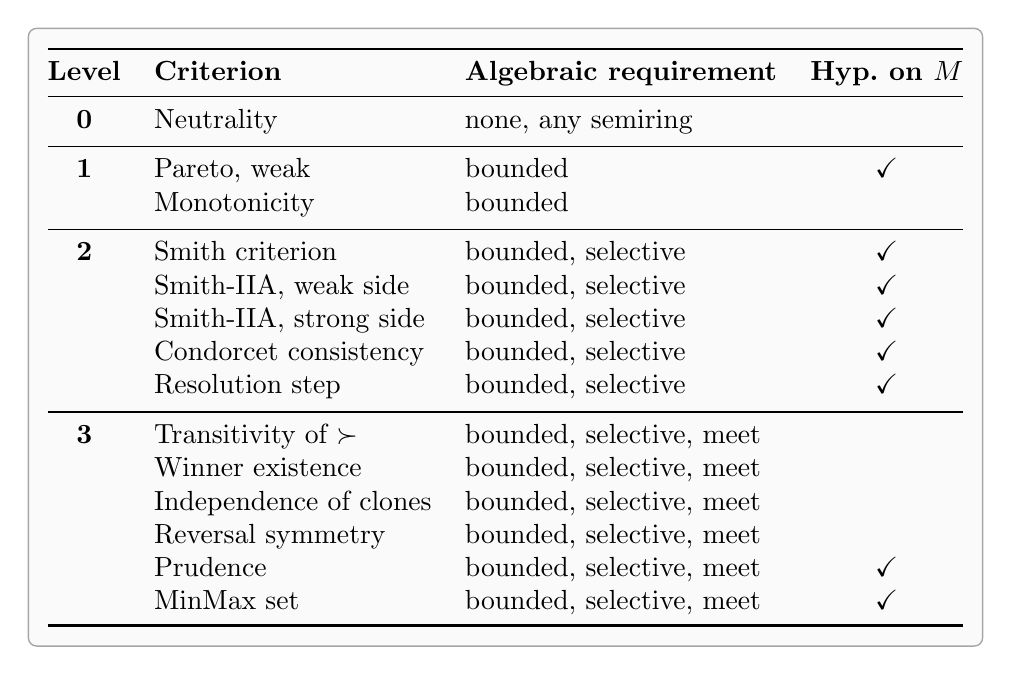
\begin{tikzpicture}
\node[draw=black!35,rounded corners=3pt,line width=0.5pt,
      inner sep=7pt,fill=black!2] {%
\begin{tabular}{@{}cllc@{}}
\toprule
\textbf{Level} & \textbf{Criterion} & \textbf{Algebraic requirement} & \textbf{Hyp.\ on $M$} \\
\midrule
\textbf{0} & Neutrality                 & none, any semiring       & \\[1pt]
\midrule
\textbf{1} & Pareto, weak               & bounded                  & $\checkmark$ \\
           & Monotonicity               & bounded                  & \\[1pt]
\midrule
\textbf{2} & Smith criterion            & bounded, selective       & $\checkmark$ \\
           & Smith-IIA, weak side       & bounded, selective       & $\checkmark$ \\
           & Smith-IIA, strong side     & bounded, selective       & $\checkmark$ \\
           & Condorcet consistency      & bounded, selective       & $\checkmark$ \\
           & Resolution step            & bounded, selective       & $\checkmark$ \\[1pt]
\midrule
\textbf{3} & Transitivity of $\succ$    & bounded, selective, meet & \\
           & Winner existence           & bounded, selective, meet & \\
           & Independence of clones     & bounded, selective, meet & \\
           & Reversal symmetry          & bounded, selective, meet & \\
           & Prudence                   & bounded, selective, meet & $\checkmark$ \\
           & MinMax set                 & bounded, selective, meet & $\checkmark$ \\
\bottomrule
\end{tabular}};
\end{tikzpicture}
\caption{The criteria and their levels. Each row gives the weakest
structure under which we can establish the criterion; levels $0$ to $3$
stack, each adding one axiom to the one below. A tick in the last column
marks a criterion whose theorem also carries a hypothesis on the matrix
$M$ rather than on the semiring; except for prudence and the MinMax set,
the ballot layer derives that hypothesis from a premise about ballots. At
Level 3 the two axioms are also necessary (\Cref{sec:characterisation}).}
\label{tab:classification}
\end{table}


\subsection{Level 0: Any Semiring}

One criterion needs no algebraic assumption whatsoever.

\begin{theorem}[Neutrality]\label{thm:neutrality}
Let $\sigma$ be a permutation of $A$ and put
$M^{\sigma}_{ab} = M_{\sigma a\,\sigma b}$. Then $a \succ_{M^{\sigma}} b$ if
and only if $\sigma a \succ_{M} \sigma b$, and $a \in \mathcal{S}(M^{\sigma})$
if and only if $\sigma a \in \mathcal{S}(M)$.
\proofat{algorithm/NeutralityN.v}{neutrality\_beats, neutrality\_winner}
\end{theorem}

Neutrality reduces to the invariance of a finite sum under a permutation
of the index set: the closure respects the permutation term by term. It
needs neither boundedness nor idempotence, and it is the only criterion we
prove at the bare semiring level.

\subsection{Level 1: Boundedness}

Two criteria need boundedness, $1 + a = 1$, and nothing beyond it. By
\Cref{lem:natural} it forces $a \cdot b \leq a$ and $a \cdot b \leq b$, so
a path is never stronger than any of its links. Both proofs below rest on
two consequences: the series closes at $M^{n-1}$, so bounding a closure
entry means bounding every power, and the closure is monotone in the
matrix, so raising an entry of $M$ lowers no entry of $\Mstar$.

\begin{theorem}[Weak Pareto]\label{thm:pareto}
Let $a \neq b$, let $M$ have diagonal $1$, and suppose
$M_{ba} \leq M_{ab}$, and that
$M_{bx} \leq M_{ax}$ and $M_{xa} \leq M_{xb}$ for every
$x \notin \{a,b\}$. Then $\Mstar_{ba} \leq \Mstar_{ab}$, and consequently
$b \in \mathcal{S}(M)$ implies $a \in \mathcal{S}(M)$.
\proofat{algorithm/ParetoN.v}{pareto\_weaker}
\end{theorem}

The hypotheses say that $a$ dominates $b$ head to head and against every
third alternative. They constrain the matrix, not the semiring, and the
ballot layer derives them from the premise that every voter ranks $a$ at
least as high as $b$.

\begin{theorem}[Monotonicity]\label{thm:monotone}
Let $M'$ be obtained from $M$ by raising $a$'s row and lowering $a$'s
column: $M_{ay} \leq M'_{ay}$ for every $y$, $M'_{xa} \leq M_{xa}$ for every
$x$, and $M_{xy} = M'_{xy}$ whenever $x \neq a$ and $y \neq a$. Then
$a \succ_M b$ implies $a \succ_{M'} b$, and consequently
$a \in \mathcal{S}(M)$ implies $a \in \mathcal{S}(M')$: a winner stays a
winner when it is raised.
\proofat{algorithm/MonotonicityN.v}{winner\_monotonicity}
\end{theorem}

Two independence facts drive this. The closure out of $a$ does not depend on
the edges into $a$, and the closure into $a$ does not depend on the edges out
of $a$; both hold because a walk through $a$ is dominated by the part of
itself that avoids $a$. Raising $a$'s row and lowering its column therefore
moves $\Mstar_{ab}$ up and $\Mstar_{ba}$ down, and a strict victory survives
along
\[
  (M')^{\ast}_{ba} \;\leq\; \Mstar_{ba} \;<\; \Mstar_{ab} \;\leq\;
  (M')^{\ast}_{ab},
\]
where $a \succ_M b$ supplies the strict middle step; a tie would leave it
non-strict and the chain of inequalities would conclude nothing. The winner clause applies
the same two facts to each rival in turn. All of this concerns $a$ alone:
raising $a$ may unseat some other winner, and indeed
$\mathcal{S}(M') \subseteq \mathcal{S}(M)$.



\subsection{Level 2: Selectivity}

Selectivity, $x + y \in \{x,y\}$, is exactly totality of the natural order.
It licenses one inference, and every criterion at this level uses it:
from \emph{$b$ does not beat $a$} to \emph{$a$ beats $b$}. Under a partial
order these are not complementary, since $\Mstar_{ab}$ and $\Mstar_{ba}$
may be incomparable and neither alternative beat the other. Under a total
order one of the two comparisons must hold, so a proof may split on which.

The first four theorems have one shape. A threshold $c$ cuts the
alternatives into a strong block and a weak one: every link from strong to
weak reaches $c$, and every link back falls short of it. Selectivity
converts that gap between direct links into a strict comparison of closure
entries, which is what \Cref{def:succ} reads as a win. The threshold is
Schulze's tie strength, since a victory outranks a tie and a tie outranks
a defeat. No construction on the semiring can supply it, because it turns
on $M_{ab}$ and $M_{ba}$ being read off one pair of counts; the ballot
layer discharges it.

\begin{theorem}[Smith criterion]\label{thm:smith}
Let $B_1, B_2$ partition $A$ with $B_1 \neq \emptyset$, and suppose there is
a strength $c$ with $M_{ba} < c \leq M_{ab}$ for all $a \in B_1$ and
$b \in B_2$. Then $a \succ b$ for every $a \in B_1$ and $b \in B_2$, and
every winner lies in $B_1$.
\proofat{algorithm/SmithN.v}{smith\_criterion\_weaker}
\end{theorem}

The two halves of Smith-IIA differ in which block is disturbed. Both carry
the auxiliary hypothesis $c \leq M_{xy} + M_{yx}$, which says that for
every pair the stronger of its two directions reaches the threshold.

\begin{theorem}[Smith-IIA, weak side]\label{thm:smithiia}
Under the hypotheses of \Cref{thm:smith}, together with
$c \leq M_{xy} + M_{yx}$ for $x \neq y$ and a unit diagonal on $M$,
deleting any $d \in B_2$ leaves the winner status of every $a \in B_1$
unchanged: $a \in \mathcal{S}_{A}(M)$ if and only if
$a \in \mathcal{S}_{A \setminus \{d\}}(M)$. Since every winner lies in
$B_1$ by \Cref{thm:smith}, the winner set itself is unchanged. The whole of
$B_2$ may equally be deleted at once: for every $a \in B_1$,
$a \in \mathcal{S}_{A}(M)$ if and only if $a \in \mathcal{S}_{B_1}(M)$.
\proofat{algorithm/SmithiiaN.v}{smith\_iia\_removal}
\end{theorem}

\begin{theorem}[Smith-IIA, strong side]\label{thm:smithiiastrong}
Let $B_1, B_2$ partition $A$, and suppose there is a strength $c$ with
$M_{ba} < c$ for all $a \in B_1$ and $b \in B_2$, together with
$c \leq M_{xy} + M_{yx}$ for $x \neq y$ and a unit diagonal on $M$. Then
deleting any $d \in B_1$ leaves the beat relation on the weak block
unchanged: for all $e, f \in B_2$, \;
$e \succ^{A}_{M} f$ if and only if $e \succ^{A \setminus \{d\}}_{M} f$.
\proofat{algorithm/SmithiiaN.v}{smith\_iia\_removal\_strong\_beats}
\end{theorem}

Deleting a weak alternative leaves the winner status of every strong one
alone, so the election may as well have been run on $B_1$ from the start.
Deleting a strong alternative leaves the beat relation among the weak
ones alone, and needs only the one-sided cut $M_{ba} < c$, since nothing
about the links out of $B_1$ bears on comparisons inside $B_2$.

\begin{theorem}[Condorcet consistency]\label{thm:condorcet}
Let $a$ be a Condorcet winner of $M$, and suppose that
$M_{za} < \Mstar_{ax}$ for all $z, x \neq a$ with $z \neq x$. Then
$a \succ x$ for every $x \neq a$, and hence $\mathcal{S}(M) = \{a\}$.
\proofat{algorithm/CondorcetN.v}{condorcet\_implies\_strict\_winner\_weaker}
\end{theorem}

This is the case $B_1 = \{a\}$ of the Smith criterion, with the cut written
directly as $M_{za} < \Mstar_{ax}$, and there the conclusion sharpens to
uniqueness: a lone strong alternative beats every other, so no other can
survive.

The last theorem at this level is the step that Schulze's resolvability
argument turns on. Resolvability asks that ties be rare, and the step says
that a winner with no ties in the closure is the only winner. That
pairwise distinct link strengths force such a winner is a further result,
proved at Level 3
(\rocqfile{algorithm/CriticalLinkN.v}{distinct\_links\_unique\_winner}),
and the ballot layer lifts both to profiles.

\begin{theorem}[Resolution step]\label{thm:resolution}
Let $a \in \mathcal{S}(M)$ with $\Mstar_{ab} \neq \Mstar_{ba}$ for every
$b \neq a$. Then $a \succ b$ for every $b \neq a$, and hence
$\mathcal{S}(M) = \{a\}$.
\proofat{algorithm/ResolvabilityN.v}{untied\_winner\_unique}
\end{theorem}

\begin{proof}
By selectivity either $\Mstar_{ba} \leq \Mstar_{ab}$ or
$\Mstar_{ab} \leq \Mstar_{ba}$. The second, with the entries distinct,
would be $b \succ a$, contradicting $a \in \mathcal{S}(M)$; so the first
holds, and with the entries distinct it is $a \succ b$.
\end{proof}

\subsection{Level 3: The Meet Property}
The criteria whose proofs compose two beatpaths end to end need the meet
property in addition. A bound on $\Mstar_{ab}$ and a bound on $\Mstar_{bc}$
must be combined into a bound on their product, and only the meet property
does that. One fact about the closure is used throughout: a path from $x$
to $y$ followed by one from $y$ to $z$ is itself a path from $x$ to $z$, so
\[
  \Mstar_{xy}\cdot\Mstar_{yz} \;\leq\; \Mstar_{xz}
  \qquad \text{for all } x,y,z.
\]

\begin{theorem}[Transitivity]\label{thm:trans}
Over a bounded, selective semiring with the meet property, $\succ$ is
transitive for every $M$, hence a strict partial order. With decidable
equality on the semiring in addition, $\mathcal{S}(M) \neq \emptyset$.
\proofat{algorithm/TransitivityN.v}{schulze\_trans\_weaker\_necessary}
\end{theorem}

\begin{proof}
Assume $a \succ b$ and $b \succ c$, and put
$m = \Mstar_{ab}\cdot\Mstar_{bc}$, so $m \leq \Mstar_{ac}$. By selectivity
either $\Mstar_{ca} < \Mstar_{ac}$, which is $a \succ c$, or
$\Mstar_{ac} \leq \Mstar_{ca}$; suppose the latter, so $m \leq \Mstar_{ca}$.
By selectivity again and the meet property, $m$ is the smaller of
$\Mstar_{ab}$ and $\Mstar_{bc}$. If $m = \Mstar_{ab}$, then $\Mstar_{ab}$ is
below both $\Mstar_{bc}$ and $\Mstar_{ca}$, so by the meet property and
composition
$\Mstar_{ab} \leq \Mstar_{bc}\cdot\Mstar_{ca} \leq \Mstar_{ba}$, which with
$\Mstar_{ba} \leq \Mstar_{ab}$ forces equality and contradicts $a \succ b$.
If $m = \Mstar_{bc}$, the same argument with the letters shifted gives
$\Mstar_{bc} \leq \Mstar_{ca}\cdot\Mstar_{ab} \leq \Mstar_{cb}$,
contradicting $b \succ c$. The two products are taken in opposite orders,
so commutativity is never needed. Finally, a strict partial order on a
finite set has a maximal element; to find one constructively we must
decide comparisons between closure entries, and that is the only use of
decidable equality.
\end{proof}

This is Schulze's own argument: his case split is selectivity, his
identification of a composite path's strength with its weaker half is the
meet property, and nothing else about the semiring is used.

\begin{lemma}\label{lem:commfree}
On a bounded semiring the meet property forces $\cdot$ to commute.
\proofat{algorithm/SchulzeOrderN.v}{mul\_comm\_of\_meet}
\end{lemma}

\begin{proof}
By \Cref{lem:natural} both $a\cdot b$ and $b\cdot a$ are lower bounds of
$\{a,b\}$; the meet property makes each the greatest, and a greatest lower
bound is unique.
\end{proof}

Commutativity is therefore not an independent axiom of the hierarchy: any
criterion whose hypotheses contain the meet property has it for free.

Independence of clones compares two elections over different alternative
sets, using the restricted notation of \Cref{def:succ}.

\begin{definition}[Clone replacement]\label{def:clone}
Let $d \in A$, let $K \neq \emptyset$ be fresh alternatives disjoint from
$A$, and put $A' = (A \setminus \{d\}) \cup K$. A matrix $N$ over $A'$ is a
\emph{clone replacement} of $d$ by $K$ in $M$ when, for all
$a, b \in A \setminus \{d\}$ and $g \in K$,
\[
  N_{ga} = M_{da}, \qquad N_{ag} = M_{ad}, \qquad N_{ab} = M_{ab}.
\]
Each clone inherits the links of $d$ and the links among survivors are
untouched; nothing is required of $N_{gh}$ for $g, h \in K$. Both matrices
carry $1$ on the diagonal, which costs nothing since $M$ and $M \oplus I$
have the same star.
\proofat{algorithm/CloneN.v}{CloneN.v}
\end{definition}

\begin{theorem}[Independence of clones]\label{thm:clones}
Over a bounded semiring, let $N$ be a clone replacement of $d$ by $K$ in
$M$. Then for every $a \in A \setminus \{d\}$,
$a \in \mathcal{S}_{A}(M)$ if and only if $a \in \mathcal{S}_{A'}(N)$. If
the semiring is moreover selective with the meet property and decidable
equality, then $d \in \mathcal{S}_{A}(M)$ if and only if
$\mathcal{S}_{A'}(N) \cap K \neq \emptyset$.
\proofat{algorithm/CloneN.v}{independence\_of\_clones}
\end{theorem}

\begin{proof}
The idea is that a clone set behaves, from outside, exactly like the
alternative it replaced. Three equalities of closure entries make that
precise: for all $a, b \in A \setminus \{d\}$ and $g \in K$,
\[
  \clo{N}{A'}_{ab} = \clo{M}{A}_{ab}, \qquad
  \clo{N}{A'}_{ag} = \clo{M}{A}_{ad}, \qquad
  \clo{N}{A'}_{ga} = \clo{M}{A}_{da}.
\]
Each is proved by antisymmetry, transporting paths in both directions:
from old to new, rename $d$ to a fixed clone $g$; from new to old, rename
every clone to $d$. The image path has its link strengths recomputed in
the target matrix, so it is a path by construction and only a link-by-link
comparison remains. Crossings between $K$ and the survivors are equalities
by \Cref{def:clone}. A path that enters $K$ and leaves it again is
collapsed onto $d$, where the recomputed link is $M_{dd} = 1$, which
dominates whatever the clones did among themselves; this is the only use
of boundedness.

The first clause follows from the equalities alone: a survivor $b$ beats
$a$ in one election exactly when it does in the other, and a clone $g$
beats $a$ in the new election exactly when $d$ beat $a$ in the old. For the
second, if some survivor beat $d$ then by the equalities it beats every
clone, so no clone wins. If none did, no survivor beats any clone, and only
other clones can; by \Cref{thm:trans} the relation is a strict partial
order, so the finite non-empty set $K$ has a maximal element, which is a
winner.
\end{proof}

Two further criteria sit at this level. \emph{Prudence} demands that a
link stronger than every directed cycle be respected by the output; the
strength of the strongest directed cycle is the join, over all links
$a \to b$, of $M_{ab} \cdot \Mstar_{ba}$. The \emph{MinMax set} is
Schulze's most characteristic property. For a non-empty proper subset
$B \subset A$, the \emph{cut} into $B$ is the join of the links $M_{xb}$
with $x \notin B$ and $b \in B$, that is, the strongest link entering $B$.
A set is \emph{cut-minimising} if no other has a strictly weaker cut, and
the MinMax set $\mathfrak{B}$ is the union of the cut-minimising sets.

\begin{theorem}[Prudence and the MinMax set]\label{thm:prudminmax}
Over a bounded, selective semiring with the meet property:
(i) if $a \neq b$ and $M_{ab}$ is strictly stronger than every directed
cycle, then $a \succ b$, so $b \notin \mathcal{S}(M)$;
(ii) with decidable equality in addition, if $a$ lies in a cut-minimising
set and $b$ lies in none, then $a \succ b$, so
$\mathcal{S}(M) \subseteq \mathfrak{B}$.
\proofat{algorithm/PrudenceN.v}{prudence}
\end{theorem}

The cycle strength and each cut are joins, so they exist in any semiring.
The minimum over all cuts need not, because the natural order has joins
but not necessarily meets. The theorem therefore takes a cut-minimising
set as a hypothesis rather than computing one. That hypothesis, and the
strongest-cycle hypothesis of prudence, are the conditions on $M$ marked
in the table for these two rows; over a total order the minimum of
finitely many cuts always exists, so on Schulze's own semiring the
hypothesis costs nothing.



\subsection{The Outlier: Commutativity}\label{sec:outlier}

One criterion does not fit the hierarchy at all. Reversing every ballot
should turn the outcome upside down, and at the level of the beat relation
that is what happens: reversal is transposition of $M$, and the closure
commutes with it.

\begin{theorem}[Reversal symmetry, relation level]\label{thm:reversal}
Over a \emph{commutative} semiring, $a \succ_M b$ if and only if
$b \succ_{M^{\mathsf{T}}} a$, where $M^{\mathsf{T}}_{ij} = M_{ji}$.
\proofat{algorithm/ReversalsymmetryN.v}{reversal\_symmetry\_O}
\end{theorem}

\begin{proof}
The closure of a transpose is the transpose of the closure,
$(M^{\mathsf{T}})^{\ast}_{ab} = \Mstar_{ba}$, because a path from $a$ to
$b$ in $M^{\mathsf{T}}$ is a path from $b$ to $a$ in $M$ read backwards
and the two have the same strength. Commutativity is exactly what lets the
product be read backwards. The comparison defining $\succ$ then swaps with
it.
\end{proof}

Neither boundedness nor selectivity is used, so this sits outside the
hierarchy rather than at a level of it: the axiom it uses is one no other
criterion needs. It is not, however, an extra assumption in practice. By
\Cref{lem:commfree} the meet property already forces commutativity, so any
semiring that reaches Level 3 has it for free, and the same statement
holds there with no commutativity hypothesis at all.
\proofat{algorithm/ReversalsymmetryN.v}{reversal\_symmetry\_O\_level2}

The winner-level forms of reversal symmetry, that a reversal displaces a
winner exactly when it promotes a non-winner, and that the winner set is
unchanged only when everything was tied, do need the full Level 3
apparatus, which is why they appear there in \Cref{tab:classification}.
\rocqrelated{\rocqfile{algorithm/ReversalsymmetryN.v}{reversal\_symmetry\_S}, and
\rocqfile{algorithm/ReversalsymmetryN.v}{reversal\_\allowbreak symmetry\_all\_tied}}

\section{The Top of the Hierarchy is Exact}\label{sec:characterisation}

\Cref{thm:trans} says selectivity and the meet property suffice for
transitivity. This section shows they are necessary, so that the Level 3
row of \Cref{tab:classification} states a characterisation rather than a
sufficient condition. It then shows, with two concrete semirings, that
each axiom is necessary on its own and that the cardinality bounds in the
characterisations cannot be improved.

We first record what the two axioms do to the semiring. They already force
multiplication to commute (\Cref{lem:commfree}), and in fact they pin both
operations completely.

\begin{proposition}[Structure]\label{thm:structure}
A bounded semiring that is selective and has the meet property is a
\emph{bottleneck semiring}: its natural order is total, with least element
$0$ and greatest element $1$; $+$ is the join $\max$ of that order, and
$\cdot$ is the meet $\min$.
\proofat{algorithm/SchulzeOrderN.v}{structure\_add\_is\_max,
structure\_mul\_is\_min}
\end{proposition}

\begin{proof}
Selectivity says the order is total, and \Cref{lem:natural}
identifies its extremes and shows $+$ is the join, which in a total order is
$\max$. The meet property makes $a\cdot b$ the greatest lower bound, which
in a total order is $\min$. 
\end{proof}


\begin{theorem}[Transitivity Characterisation]\label{thm:characterisation}
Let $R$ be a bounded semiring with decidable equality and let $|A| \geq 3$.
Then
\[
  \succ_M \text{ is transitive for every } M
  \quad\Longleftrightarrow\quad
  R \text{ is selective and has the meet property,}
\]
and hence, by \Cref{thm:structure}, if and only if $R$ is a bottleneck
semiring.
\proofat{algorithm/TransitivityN.v}{transitivity\_\allowbreak characterisation}
\end{theorem}

\begin{proof}
Right to left is \Cref{thm:trans}. For the converse, assume $\succ_M$ is
transitive for every $M$ and fix three distinct alternatives $X, Y, Z$.

Everything rests on one construction. For $p, q, r \in R$ let $T(p,q,r)$ be
the matrix on $\{X,Y,Z\}$ with exactly three links, $X \to Y$ of strength $p$,
$Y \to Z$ of strength $q$, and $Z \to X$ of strength $r$, and $0$ everywhere
else. The only route from $Y$ back to $X$ is $Y \to Z \to X$, of strength
$q \cdot r$, so
$q \cdot r < p$ makes $X \succ Y$; likewise $r \cdot p < q$ makes
$Y \succ Z$. Transitivity then forces $X \succ Z$. But the only route from
$X$ to $Z$ is $X \to Y \to Z$, so the closure entry $T^{\ast}_{XZ}$ is at
most $p \cdot q$, while the direct link gives $r \leq T^{\ast}_{ZX}$.
Chaining the three facts,
\[
  q \cdot r < p \;\text{ and }\; r \cdot p < q
  \qquad\Longrightarrow\qquad
  r < p \cdot q .
\]
Call this the \emph{triangle test}. It converts two strict comparisons into
a third, and both halves of the proof are applications of it.

\emph{Selectivity.} Suppose $x$ and $y$ were incomparable, so neither
$x \leq y$ nor $y \leq x$. Run the test on $p = x$, $q = y$, $r = x \cdot y$.
Its premises hold: $y \cdot (x \cdot y)$ lies below $x$, and it cannot equal
$x$, since it also lies below $y$ and that would give $x \leq y$;
symmetrically $(x \cdot y) \cdot x$ lies strictly below $y$. The test
concludes $x \cdot y < x \cdot y$, which is absurd. So no incomparable pair
exists, and the natural order is total, which is selectivity.

\emph{Meet property.} Let $m \leq a$ and $m \leq b$, and suppose
$m \not\leq a \cdot b$. Run the test on $p = a$, $q = b$, $r = m$. Its two
premises ask that $b \cdot m$ lie strictly below $a$ and $m \cdot a$
strictly below $b$; the non-strict parts are immediate, since
$b \cdot m \leq m \leq a$ and $m \cdot a \leq m \leq b$. If both are strict
the test gives $m \leq a \cdot b$, contradicting the supposition. Otherwise
one of them is an equality. If $b \cdot m = a$ then $a = m$, and running the
test instead on the triangle $(b, m, m)$ contradicts that equality; the case
$m \cdot a = b$ is symmetric. So $m \leq a \cdot b$ in every case.

Decidable equality is used only in this direction. Both conclusions are
decidable statements, and each is reached by refuting its negation.
\end{proof}



\begin{theorem}[Winner existence]\label{thm:winnerchar}
Let $R$ be a bounded semiring with decidable equality and let $|A| \geq 4$.
Then $\mathcal{S}(M) \neq \emptyset$ for every $M$ if and only if $R$ is
selective and has the meet property.
\proofat{algorithm/WinnerexistenceN.v}{winner\_exists\_\allowbreak characterisation}
\end{theorem}

\begin{proof}
Right to left is \Cref{thm:trans}. The converse needs two witnesses rather
than one: a square on four alternatives for selectivity, and then the
familiar triangle for the meet property. The triangle alone will not do,
which is why the bound here is four and not three.

\emph{Selectivity.} Suppose $x$ and $y$ are incomparable. Then
$x \cdot y < y$ and $y \cdot x < x$: each product lies below both factors,
and equality either way would make $x$ and $y$ comparable. Build the
\emph{square} $S(x,y)$ on four alternatives $A, B, C, D$, with four links
$B \to A$ and $D \to C$ of strength $x$, and $A \to D$ and $C \to B$ of strength $y$,
and $0$ elsewhere. Each alternative has exactly one route back to the one
in front of it, and that route has strength $x\cdot y$ or $y \cdot x$, so it
loses. The four beats close into a cycle, no alternative is unbeaten, and
$\mathcal{S}(S(x,y)) = \emptyset$. So there is no incomparable pair.

\emph{Meet property.} With selectivity in hand the triangle suffices, on
three alternatives. Let $m \leq a$ and $m \leq b$ with
$m \not\leq a\cdot b$, and replace $m$ by $m + a\cdot b$, which still lies
below $a$ and $b$ but now has $a \cdot b$ strictly below it. The triangle on
$(a,\, b,\, m + a\cdot b)$ then has all three of its links beating their
return routes, so its beat relation is a strict cycle and again no
alternative wins.
\end{proof}

\Cref{sec:sharp} shows that four alternatives are needed here, not merely
convenient.

\begin{corollary}[Well-formed output]\label{thm:outputchar}
Let $R$ be a bounded semiring with decidable equality. For $|A| \geq 3$,
$\succ_M$ is a strict partial order for every $M$, and Schulze's stated
output, a strict partial order together with a non-empty winner set, is
delivered for every $M$, if and only if $R$ is selective and has the meet
property. For $|A| \geq 4$ the same holds of the property that every
non-winner is beaten by some winner.
\proofat{algorithm/CharacterisationsN.v}{output\_well\_formed\_\allowbreak characterisation}
\end{corollary}

\begin{proof}
A strict partial order is in particular transitive, so
\Cref{thm:characterisation} gives the axioms from the first two
properties, and three alternatives suffice because the transitivity
component supplies the converse on its own. If every non-winner is beaten
by a winner then a winner exists, so refuting the last property means
refuting winner existence, which needs the four alternatives of
\Cref{thm:winnerchar}.
\end{proof}

\begin{theorem}[Independence of clones]\label{thm:clonechar}
Let $R$ be a bounded semiring with decidable equality and let $|A| \geq 5$.
Then \Cref{thm:clones} holds for every clone replacement if and only if $R$
is selective and has the meet property. Consequently independence of clones
and winner existence are the same condition on the semiring.
\proofat{algorithm/CloneCharacterisationN.v}{clone\_characterisation, clone\_iff\_winner\_exists}
\end{theorem}

\begin{proof}
Right to left is \Cref{thm:clones}. For the converse, note that the clone
hypotheses of \Cref{def:clone} constrain nothing about the links among the
clones, and go vacuous when the old alternative set is the single
alternative $d$. There the criterion says exactly that an arbitrary matrix
on an arbitrary non-empty set of clones has an undefeated element, which is
winner existence. The square and the triangle of \Cref{thm:winnerchar} can
therefore be replayed inside the clone set, with the replaced alternative
parked outside as a node no link leaves; that spare node is why five
alternatives are asked for rather than four. The equivalence with winner
existence is then immediate, since both sides characterise the same pair of
axioms.
\end{proof}

Independence of clones is the criterion Schulze's method is best known
for, and in this setting it is not an extra demand at all: a semiring that
always returns a winner is automatically clone-independent, and
conversely.

\begin{figure}[t]
\centering
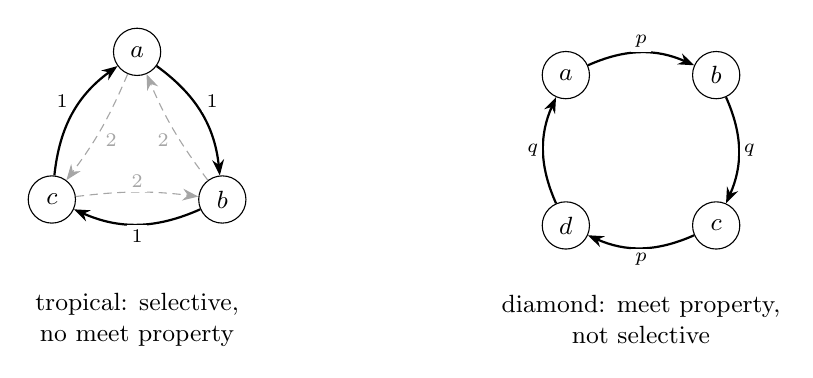
\begin{tikzpicture}[
  >={Stealth[length=2mm]},
  nd/.style={circle,draw,minimum size=6mm,inner sep=0pt,font=\small},
  fwd/.style={->,thick,bend left=24},
  bwd/.style={->,densely dashed,gray!70,bend left=7},
  every node/.style={font=\scriptsize,inner sep=1.5pt,fill=white},
  capt/.style={font=\small,fill=none,align=center}]

  \begin{scope}
    \node[nd] (a) at (90:1.25)  {$a$};
    \node[nd] (b) at (330:1.25) {$b$};
    \node[nd] (c) at (210:1.25) {$c$};
    \draw[fwd] (a) to node[auto] {$1$} (b);
    \draw[fwd] (b) to node[auto] {$1$} (c);
    \draw[fwd] (c) to node[auto] {$1$} (a);
    \draw[bwd] (b) to node[auto] {$2$} (a);
    \draw[bwd] (c) to node[auto] {$2$} (b);
    \draw[bwd] (a) to node[auto] {$2$} (c);
    \node[capt] at (0,-2.15) {tropical: selective,\\ no meet property};
  \end{scope}

  \begin{scope}[xshift=6.4cm]
    \node[nd] (A) at (135:1.35) {$a$};
    \node[nd] (B) at (45:1.35)  {$b$};
    \node[nd] (C) at (315:1.35) {$c$};
    \node[nd] (D) at (225:1.35) {$d$};
    \draw[fwd] (A) to node[auto] {$p$} (B);
    \draw[fwd] (B) to node[auto] {$q$} (C);
    \draw[fwd] (C) to node[auto] {$p$} (D);
    \draw[fwd] (D) to node[auto] {$q$} (A);
    \node[capt] at (0,-2.15) {diamond: meet property,\\ not selective};
  \end{scope}
\end{tikzpicture}
\caption{The two witnesses. Left, over the tropical semiring, forward hops
cost $1$ and return hops $2$; the closure preserves the asymmetry, so the
beats form a $3$-cycle and no alternative is unbeaten. Right, over the
diamond, the incomparable pair $p, q$ alternates round four alternatives and
again nobody is unbeaten, whereas at three alternatives the diamond always
produces a winner. Each semiring drops exactly one Level 3 axiom, so
neither axiom can be dropped in favour of the other.}
\label{fig:witnesses}
\end{figure}

\subsection{Neither Axiom Can Be Dropped}\label{sec:sharp}

The characterisations above say that selectivity and the meet property are
together necessary. Two semirings, each dropping exactly one of the two
axioms, show that each is necessary on its own and that the cardinality
bounds are optimal. Both are small enough to check by hand and both are
checked by machine.

\subparagraph*{The tropical semiring: selective, no meet property.}
Take $\langle \mathbb{N}^{\infty}, \min, +\rangle$, the shortest-path
semiring of \Cref{ex:tropical}. Its natural order is total, since $\min$
always returns one of its arguments, so it is selective. It fails the meet
property: $1$ is a lower bound of $\{1, 1\}$, but $1 \cdot 1 = 2$ and in
the natural order of this semiring $2$ lies strictly below $1$, so the
product is a lower bound of its factors but not the greatest one. That is
enough to break the method at three alternatives
(\Cref{fig:witnesses}, left): hops forward round a triangle cost $1$ and
hops back cost $2$, the closure leaves the asymmetry untouched, and
$a \succ b \succ c \succ a$ is a cycle of strict wins with no unbeaten
alternative. Selectivity alone therefore buys nothing at Level 3.
\proofat{examples/SharpnessWitness.v}{tropical\_no\_winner\_at\_three}

\subparagraph*{The diamond: meet property, not selective.}
Take the four-element lattice $\Diam = \{\bot, p, q, \top\}$ in which $p$
and $q$ are incomparable, with join for addition and meet for
multiplication. Multiplication is by construction the greatest lower
bound, so the meet property holds, but $p + q = \top$ is neither $p$ nor
$q$, so the semiring is not selective. The square of \Cref{thm:winnerchar},
instantiated with $p$ and $q$, gives a matrix on four alternatives whose
beat relation runs round all four (\Cref{fig:witnesses}, right), so again
nobody is unbeaten, and the meet property alone buys nothing either.
Three alternatives would not have sufficed: over $\Diam$ \emph{every}
matrix on three alternatives has a winner. There are $4^{9}$ such
matrices, and we check all of them by evaluating a boolean winner test,
proved sound against $\mathcal{S}$, on each one. The bound of four in
\Cref{thm:winnerchar} therefore cannot be lowered.
\rocqrelated{\rocqfile{examples/SharpnessWitness.v}{diamond\_no\_winner\_at\_four} and
\rocqfile{examples/SharpnessWitness.v}{diamond\_every\_profile\_has\_winner}}

\subparagraph*{Level 2 is sharp as well.}
The same diamond settles the level below. Over $\Diam$ we exhibit a matrix
with a clean threshold separating a strong block from a weak one and a
winner outside the strong block, so the Smith criterion fails; a matrix
with a Condorcet winner that the closure does not elect; a matrix in which
an untied winner is not unique, so the resolution step fails; and
matrices refuting both halves of Smith-IIA. Each is a small explicit
table, and each failure comes from two incomparable strengths, which is
precisely what selectivity forbids. So boundedness and the meet property
together are not enough for any Level 2 criterion.
\rocqrelated{\rocqfile{examples/SharpnessWitness.v}{smith\_fails\_over\_diamond},
\rocqfile{examples/SharpnessWitness.v}{condorcet\_fails\_\allowbreak over\_diamond},
\rocqfile{examples/SharpnessWitness.v}{resolution\_fails\_\allowbreak over\_diamond}, and
\rocqfile{examples/SharpnessWitness.v}{smith\_iia\_fails\_\allowbreak over\_diamond}}

\section{Formal Verification}\label{sec:formalisation}

Mechanisation does more here than certify the proofs. The hierarchy of
\Cref{sec:classification} is \emph{enforced} rather than asserted, because
each theorem carries exactly the algebra its proof uses and nothing else.
Neutrality is stated over a bare semiring, so a proof of it cannot reach
for boundedness; the Level 1 results are stated over a bounded semiring
with no further hypothesis, so they cannot quietly appeal to selectivity;
and selectivity and the meet property appear as explicit arguments of the
theorems that need them. Where the paper claims an axiom is not required,
the type checker confirms it.

The development is carried out in \rocq{}. It runs to some $20{,}000$
lines, nothing is admitted and no axiom is assumed, and the proofs are
constructive, so the definitions extract to executable OCaml.

\subparagraph*{Three base files.}
Every later file, and every example, is stated over three files.
\rocqfile{algorithm/MatN.v}{MatN.v} builds the matrix semiring over an
arbitrary semiring: a matrix is a function $A \times A \to R$, addition is
entrywise, multiplication is the usual $\sum_k M_{ik}\cdot N_{kj}$, and $I$
carries $1$ on the diagonal. Everything about powers, the geometric sum,
and their monotonicity lives here.
\rocqfile{algorithm/PathN.v}{PathN.v} gives the concrete reading of the
same objects. A path is an explicit list of links, its strength is the
product of them, and \texttt{path\_star} joins the strengths of all paths
of length below $|A|$. The two views are identified,
$\texttt{path\_star}\ M\ c\ d = \Mstar_{cd}$, so a statement proved about
powers may be read back as a statement about walks; this is how the gloss
of \Cref{sec:prelim} is discharged, and the cycle lemmas of the same file
are what justify stopping at $|A| - 1$.
\rocqfile{algorithm/SemimoduleN.v}{SemimoduleN.v} proves the standard
fixed-point facts of the algebraic path problem over an arbitrary bounded
semiring: $\Mstar b$ is the least solution of $x = M x + b$, and under
boundedness the unique one. This is what earns the closure the name
Kleene star.
\rocqrelated{\rocqfile{algorithm/SchulzeDefsN.v}{path\_star\_\allowbreak elements\_is\_mat\_star},
\rocqfile{algorithm/SemimoduleN.v}{kleene\_fixed\_point},
\rocqfile{algorithm/SemimoduleN.v}{kleene\_fixed\_\allowbreak point\_least}, and
\rocqfile{algorithm/SemimoduleN.v}{kleene\_fixed\_\allowbreak point\_unique}}

\subparagraph*{Two representations of a matrix.}
Taking a matrix to be a \emph{function} is what makes the theory pleasant:
two matrices are equal when they agree at every pair, and no bookkeeping
about lengths or well-formedness ever appears in a statement. It is also
unusable as a program, because a function memoises nothing. The
development therefore carries a second, tabulated representation as a list
of rows, on which \texttt{mul\_list} and \texttt{pow\_list} do the
arithmetic with each entry computed once; repeated squaring then computes
the closure in $O(n^{3}\log k)$. The two representations are proved to
agree, $\texttt{of\_list}\,(\texttt{pow\_list}\,(\texttt{to\_list}\ M)\ k)_{cd}
= (M^{k})_{cd}$, so the statements quantify over functions, where they read
cleanly, and the extracted program runs on lists, where it is fast.
\rocqrelated{\rocqfile{algorithm/MatN.v}{of\_list\_\allowbreak to\_list},
\rocqfile{algorithm/MatN.v}{of\_list\_\allowbreak pow\_pos\_list}, and
\rocqfile{algorithm/MatN.v}{pow\_fun\_\allowbreak powN\_fun\_eqv}}

\subparagraph*{Instances.}
Because every result is stated over an arbitrary semiring, an instance is
just a set with its two operations and a proof of the axioms.
\rocqfile{examples/Schulze.v}{Schulze.v} supplies the max-min semiring of
\Cref{sec:intro} and runs Schulze's own worked example;
\rocqfile{examples/Shortestpath.v}{Shortestpath.v} and
\rocqfile{examples/WidestShortestPath.v}{Widest\-Shortest\-Path.v} give shortest
and widest-shortest paths, and
\rocqfile{examples/FiveGNetworkSlicing.v}{FiveGNetworkSlicing.v} a product
of the two that models routing across network slices. Each extracts to
running OCaml.

\subparagraph*{Beatpaths themselves, not just their strength.}
One instance shows how little the construction depends on the numbers.
\rocqfile{examples/Schulzepath.v}{Schulzepath.v} keeps the alternatives
and the links but replaces the semiring by \emph{sets of paths}: an
element is a set of edge sequences, addition is union, multiplication
concatenates every path of the left set with every path of the right, $0$
is the empty set and $1$ the set containing only the empty path. These
satisfy the semiring axioms, so the same closure applies unchanged, and
$\Mstar_{ab}$ is now the set of all beatpaths from $a$ to $b$. The
strength is recovered afterwards, as the best measure of a path in that
set.


\section{Related Work}\label{sec:related}
\subparagraph*{Algebraic path problems.}
Carr\'e~\cite{carre1971algebra} and Lehmann~\cite{lehmann1977} showed that
transitive closure, shortest paths, and widest paths are one algorithm over
different semirings, and Gondran and Minoux~\cite{10.5555/1386688} and Baras
and Theodorakopoulos~\cite{baras2022path} developed the
idea. Mohri~\cite{10.5555/639508.639512},
Dolan~\cite{10.1145/2500365.2500613} and Droste and
Kuich~\cite{Droste2009} are standard modern presentations. That literature
asks when the series converges and how to compute it
efficiently~\cite{vassilevska2009all}, not when the values may be
\emph{compared}, which is the question a voting rule puts to it. Bottleneck
semirings are classical, going back to Cuninghame-Green's minimax
algebra~\cite{cuninghamegreen1979minimax}. On the computational side,
Sornat, Vassilevska Williams, and Xu~\cite{sornat2021schulze} give
fine-grained bounds for computing Schulze winners via a reduction to
all-pairs bottleneck paths, and Csar, Lackner, and
Pichler~\cite{csar2018computing} compute the method at scale in the Pregel
model, again by working with bottleneck paths on the pairwise graph. Both
take that structure as a convenient route to an algorithm;
\Cref{thm:structure} explains why it is not one route among many but the
only shape the problem can take.


\subparagraph*{Algebraic conditions as the price of a guarantee.}
Asking which algebraic hypothesis buys which property is established in the
theory of routing metrics~\cite{10.1145/3387514.3405864}. Daggitt, Gurney,
and Griffin's Agda development of asynchronous convergence for Bellman-Ford
protocols~\cite{10.1145/3230543.3230561} is the closest methodological
neighbour: a mechanised, algebra-parameterised account where the hypotheses
are exactly the price of the guarantee. The same style has reached
model-theoretic preservation properties~\cite{brinke2026}, and semiring
provenance is where a construction's dependence on its algebra is studied
most systematically~\cite{10.1145/1265530.1265535,10.5555/3319379.3319390}.
Our results have the same shape, with a social choice guarantee in place of
a protocol or a logic, and with the correspondence closed to an
equivalence.

\subparagraph*{Mechanised algebra and verified social choice.}
Kleene algebra has been mechanised as a decision
procedure~\cite{10.1007/978-3-642-14052-5_13,MOREIRA2015377}, and functional
presentations of closure over semirings are
known~\cite{10.1007/978-3-319-17822-6_14}. Our development differs in how it
is organised. Because our claims concern minimality of hypotheses, each
theorem is stated at the weakest level of the hierarchy that supports it. On the
social choice side, formalisations of impossibility
theorems~\cite{arrow1950difficulty,nipkow2009social} and verified vote counting, including for
the Schulze method, are well
established~\cite{10.1007/978-3-319-66107-0_26,ghale2018modular,10.1007/978-3-030-03592-1_5}.
That work verifies a particular procedure over a fixed semiring. Closest to the
present paper is Tiwari and Pattinson's machine-checked proof that a
\rocq{} implementation of the Schulze method satisfies the Condorcet winner
criterion~\cite{tiwari2021machine}, which leaves reversal symmetry, Pareto,
monotonicity and the rest explicitly as future work. Our concern is
complementary to all of it: rather than certifying one procedure against one
criterion, we ask how much algebraic structure each criterion costs, and
answer it for the whole family at once. 

\section{Conclusion}\label{sec:conclusion}

We set out to ask, for each of Schulze's guarantees, how much arithmetic
its proof really needs, and the answer is that the guarantees are not a
flat list. Neutrality holds over any semiring. Weak Pareto and
monotonicity need only that the empty path is unbeatable. The Smith
criterion and Condorcet consistency need in addition that any two
strengths are comparable. The guarantees that join two beatpaths end to
end need one thing more, that the strength of a composite path is the
weaker of its halves.

At the top the levels are not merely sufficient but exact. Transitivity of
the outranking relation, existence of a winner, and independence of clones
each hold for every profile precisely when the semiring is selective and
has the meet property, and a semiring with those two properties is $\max$
and $\min$ on a total order. So the operations Schulze chose are the only
ones that work, and the only freedom left is the scale on which strengths
are recorded. We did not expect independence of clones, the criterion the
method is best known for, to turn out to be the same condition on the
semiring as the bare existence of a winner. The story is not uniformly
tidy, however. Several criteria carry conditions that no choice of
semiring can supply, because they are conditions on the ballots rather
than on the algebra, and a separate ballot layer discharges those from
Schulze's own premises.

\bibliography{ref,icalp}

\end{document}
